\section{ТЕОРЕТИЧЕСКИЕ СВЕДЕНИЯ}

Протокол IP, входящий в группу протоколов TCP/IP \textit{(Transmission Control Protocol /
Internet Protocol)}, является одним из ключевых элементов, обеспечивающих
передачу данных между узлами всемирной паутины. На сегодняшний день в интернете
наиболее распространена версия протокола IPv4. Ожидается, что на смену IPv4
в скором времени должен прийти более совершенный IPv6.

Протокол IP определяет адресацию сетевых узлов в Интернете и способы
фрагментации передаваемых по каналам связи пакетов данных.

Для того чтобы узлы сети смогли обмениваться данными, они должны получить
специальное <<имя>> --- уникальный идентификатор, называемый IP-адресом,
формат которого определяется протоколом IP. Грубо говоря, IP-адрес позволяет
отличить один узел от другого. В IPv4 адрес состоит из 32 бит и обычно
записывается в виде четырех чисел, разделенных точками. Пример IPv4 адреса: 192.168.11.17.
Каждый IP-адрес включает в себя две части: \textit{номер сети} и
\textit{номер узла} в этой сети.
То есть IP-адрес компьютера идентифицирует и компьютерную сеть,
в которую входит данный компьютер (в качестве узла), и сам этот компьютер.
Понять, какая часть IP-адреса определяет номер сети, а какая --- номер узла,
позволяют значения специальных битов адреса.
Пример разбиения IP адреса на адрес сети и адрес узла показан на
рисунке~\ref{pic:ipnethostmiddle}
\begin{figure}[h!]
  \centering
  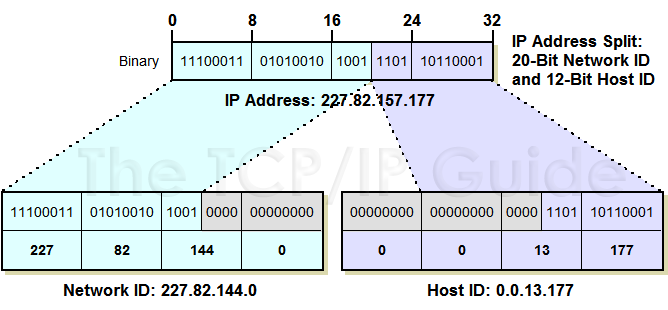
\includegraphics[width=0.8\linewidth]{pic/ipnethostmiddle}
  \caption{Разбиения IP адреса на адрес сети и адрес узла}
  \label{pic:ipnethostmiddle}
\end{figure}

Адресное пространство IP в Интернете ограничено, а его распределение --- одна из функций,
которую координирует корпорация \textit{ICANN}. ICANN, с помощью специальной процедуры,
передаёт блоки IP-адресов, выделенных из общего пространства адресов Интернета,
региональным интернет-регистратурам (RIR). Далее адреса распределяются между
организациями, представляющими RIR в каждой стране региона. Те, в свою очередь,
передают их интернет-провайдерам, которые, в конечном итоге,
делегируют их конечным потребителям.

Протокол IP является ненадежным протоколом без установления соединения.
Это означает, что протокол IP не подтверждает доставку данных,
не контролирует целостность полученных данных и не производит операцию
\textit{квитирования (handshaking)} --- обмена служебными сообщениями,
подтверждающими установку соединения с узлом назначения и его готовность
к приему данных. Протокол IP обрабатывает каждую дейтаграмму как независимую
единицу, не имеющую связи ни с какими другими дейтаграммами в Интернет.
После того, как дейтаграмма отправляется в сеть, ее дальнейшая судьба
никак не контролируется отправителем (на уровне протокола IP).
Если дейтаграмма не может быть доставлена, она уничтожается.
Узел, уничтоживший дейтаграмму, может оправить по обратному
адресу ICMP-сообщение о причине сбоя.

Гарантию правильной передачи данных предоставляют протоколы вышестоящего уровня (например, протокол TCP), которые имеют для этого необходимые механизмы.

Одна из основных задач, решаемых протоколом IP, --- маршрутизация дейтаграмм,
то есть определение пути следования дейтаграммы от одного узла сети
к другому на основании адреса получателя.

Общий сценарий работы модуля IP на каком-либо узле сети,
принимающего дейтаграмму из сети, таков:
\begin{itemize}
  \item с одного из интерфейсов уровня доступа к среде передачи (например,
    с Ethernet-интерфейса) в модуль IP поступает дейтаграмма;
  \item модуль IP анализирует заголовок дейтаграммы;
  \item если пунктом назначения дейтаграммы является данный компьютер, то проверяется,
    если дейтаграмма является фрагментом большей дейтаграммы,
    ожидаются остальные фрагменты, после чего из них собирается
    исходная большая дейтаграмма. Из дейтаграммы извлекаются данные
    и направляются на обработку одному из протоколов вышележащего
    уровня (какому именно --- указывается в заголовке дейтаграммы);
  \item если дейтаграмма не направлена ни на один из IP-адресов данного узла,
    то дальнейшие действия зависят от того, разрешена или запрещена
    ретрансляция (forwarding) “чужих” дейтаграмм;
  \item если ретрансляция разрешена, то определяются следующий узел сети,
    на который должна быть переправлена дейтаграмма для доставки ее по назначению,
    и интерфейс нижнего уровня, после чего дейтаграмма передается
    на нижний уровень этому интерфейсу для отправки;
    при необходимости может быть произведена фрагментация дейтаграммы;
  \item если же дейтаграмма ошибочна или по каким-либо причинам не может быть
    доставлена, она уничтожается; при этом, как правило, отправителю
    дейтаграммы отсылается ICMP-сообщение об ошибке.
\end{itemize}

При получении данных от вышестоящего уровня для отправки их по сети IP-модуль
формирует дейтаграмму с этими данными, в заголовок которой заносятся
адреса отправителя и получателя (также полученные от транспортного уровня)
и другая информация; после чего выполняются следующие шаги:
\begin{itemize}
  \item если дейтаграмма предназначена этому же узлу, из нее извлекаются данные
    и направляются на обработку одному из протоколов транспортного
    уровня (какому именно --- указывается в заголовке дейтаграммы);
  \item если дейтаграмма не направлена ни на один из IP-адресов данного узла,
    то определяются следующий узел сети, на который должна быть переправлена
    дейтаграмма для доставки ее по назначению, и интерфейс нижнего уровня,
    после чего дейтаграмма передается на нижний уровень этому интерфейсу для отправки;
    при необходимости может быть произведена фрагментация дейтаграммы;
  \item если же дейтаграмма ошибочна или по каким-либо причинам не может быть доставлена, она уничтожается.
\end{itemize}

\textit{Узлом сети} называется компьютер, подключенный к сети и поддерживающий
протокол IP. Узел сети может иметь один и более IP-интерфейсов, подключенных
к одной или разным сетям, каждый такой интерфейс идентифицируется уникальным IP-адресом.

\textit{IP-сетью} называется множество компьютеров (IP-интерфейсов), часто,
но не всегда подсоединенных к одному физическому каналу связи, способных
пересылать IP-дейтаграммы друг другу непосредственно (то есть без ретрансляции
через промежуточные компьютеры), при этом IP-адреса интерфейсов одной IP-сети
имеют общую часть, которая называется адресом, или номером, IP-сети,
и специфическую для каждого интерфейса часть, называемую адресом, или номером,
данного интерфейса в данной IP-сети.

\textit{Маршрутизатором}, или \textit{шлюзом}, называется узел сети с
несколькими IP-интерфейсами, подключенными к разным IP-сетям,
осуществляющий на основе решения задачи маршрутизации перенаправление
дейтаграмм из одной сети в другую для доставки от отправителя к получателю.

\textit{Хостами} называются узлы IP-сети, не являющиеся маршрутизаторами.
Обычно хост имеет один IP-интерфейс (например, связанный с сетевой картой
Ethernet или с модемом), хотя может иметь и несколько.
